
\documentclass[aspectratio=169]{beamer}

% --- Theme / packages ---
% -------------------------------------------------
% Packages
% -------------------------------------------------
\usepackage{amsmath, amsfonts}
\usepackage{graphicx}
\usepackage{booktabs}
\usepackage{hyperref}
\usepackage{bm}
\usepackage{siunitx}
\usepackage{listings}

% Figure search paths (relative to tex/lectures/)
\graphicspath{{../figures/lectures/}{../figures/shared/}}

% -------------------------------------------------
% Notes (speaker notes)
% -------------------------------------------------
\usepackage{pgfpages}
% Uncomment ONE of these for speaker notes:
% \setbeameroption{show notes} % notes only (for printing notes)
% \setbeameroption{show notes on second screen=right} % slides + notes

% -------------------------------------------------
% TikZ
% -------------------------------------------------
\usepackage{tikz}
\usetikzlibrary{matrix, calc}
\usepackage{xcolor} % (tikz loads xcolor, but explicit is fine)
\usetikzlibrary{arrows.meta, decorations.pathreplacing}


% -------------------------------------------------
% Themes
%--------------------------------------------------
\usetheme{default}
\usecolortheme{default}
\setbeamertemplate{navigation symbols}{}

% -----------------------------
% Code formatting
% -----------------------------
\definecolor{codegray}{RGB}{245,245,245}

\lstset{
  backgroundcolor=\color{codegray},
  basicstyle=\ttfamily\small,
  frame=single,
  breaklines=true,
  showstringspaces=false
}

% --- Shortcuts ---
%\newcommand{\dd}{\,\mathrm{d}}
\newcommand{\Grad}{\nabla}
\newcommand{\Div}{\nabla\!\cdot}
\newcommand{\bx}{\bm{x}}
\newcommand{\bn}{\bm{n}}
\newcommand{\bq}{\bm{q}}

%==========================
% Flipbook macro (put in preamble or before frames)
%==========================
\newcommand{\GSFlipFrame}[2]{%
\begin{frame}{Gauss--Seidel sweep (current point $(#1,#2)$)}
\centering
\hspace{3.5cm}
\vspace{3cm}
\begin{tikzpicture}[scale=2.2, every node/.style={font=\small}]
  % -----------------------------
  % USER SETTINGS
  % -----------------------------
  \def\Nx{6}   % i = 0..Nx-1
  \def\Ny{4}   % j = 0..Ny-1

  % current stencil location (interior)
  \def\ci{#1}
  \def\cj{#2}

  % Point spacing
  \def\s{0.85}

  % -----------------------------
  % STYLES
  % -----------------------------
  \tikzset{
    gpG/.style={circle, fill=green!70!black, inner sep=1.1pt},
    gpR/.style={circle, fill=red!75!black,   inner sep=1.1pt},
    gpbG/.style={circle, fill=green!70!black, inner sep=1.5pt},
    gpbR/.style={circle, fill=red!75!black,   inner sep=1.5pt},
    gpc/.style={circle, fill=blue, inner sep=1.7pt},
    stline/.style={dashed, thick},
    labij/.style={font=\normalsize},
    labp/.style={font=\scriptsize, text=gray!70},
  }

  % -----------------------------
  % OUTER RECTANGLE (domain)
  % -----------------------------
  \draw[thick] (0,0) rectangle ({(\Nx-1)*\s},{(\Ny-1)*\s});

  % -----------------------------
  % GRID POINTS + LABELS
  % -----------------------------
  \foreach \j in {0,...,\numexpr\Ny-1\relax} {
    \foreach \i in {0,...,\numexpr\Nx-1\relax} {

      \pgfmathsetmacro{\x}{\i*\s}
      \pgfmathsetmacro{\y}{\j*\s}

      % global index p = i + j*Nx (as in your first figure)
      \pgfmathtruncatemacro{\p}{\i + \j*\Nx}

      % boundary?
      \pgfmathtruncatemacro{\isB}{ (\i==0) || (\i==\Nx-1) || (\j==0) || (\j==\Ny-1) }
      % current center?
      \pgfmathtruncatemacro{\isC}{ (\i==\ci) && (\j==\cj) }

      % "already updated" (GS ordering): j<cj OR (j==cj and i<ci)
      \pgfmathtruncatemacro{\isUpdated}{ (\j<\cj) || ((\j==\cj) && (\i<\ci)) }

      % FORCE left boundary (i==0) and bottom boundary (j==0) to be green
      \pgfmathtruncatemacro{\forceGreen}{ \isB }

      % decide color state:
      % - center: blue
      % - else green if forced green OR updated
      % - else red
      \ifnum\isC=1
        \node[gpc] (P\i\j) at (\x,\y) {};
      \else
        \pgfmathtruncatemacro{\isGreen}{ (\forceGreen==1) || (\isUpdated==1) }
        \ifnum\isB=1
          \ifnum\isGreen=1
            \node[gpbG] (P\i\j) at (\x,\y) {};
          \else
            \node[gpbR] (P\i\j) at (\x,\y) {};
          \fi
        \else
          \ifnum\isGreen=1
            \node[gpG] (P\i\j) at (\x,\y) {};
          \else
            \node[gpR] (P\i\j) at (\x,\y) {};
          \fi
        \fi
      \fi

      % Labels (i,j) above-right; p below-right
      \node[labij, anchor=south west] at (\x+0.05,\y+0.05) {$(\i,\j)$};
      \node[labp,  anchor=north west] at (\x+0.05,\y-0.05) {$\p$};
    }
  }

  % -----------------------------
  % 5-POINT STENCIL (dashed)
  % -----------------------------
  \pgfmathsetmacro{\xc}{\ci*\s}
  \pgfmathsetmacro{\yc}{\cj*\s}

  \draw[stline] (\xc,\yc) -- ({(\ci+1)*\s},\yc);
  \draw[stline] (\xc,\yc) -- ({(\ci-1)*\s},\yc);
  \draw[stline] (\xc,\yc) -- (\xc,{(\cj+1)*\s});
  \draw[stline] (\xc,\yc) -- (\xc,{(\cj-1)*\s});

  % Mapping note
  %\node[font=\scriptsize, align=left] at ({(1)*\s+1.65},{(0)*\s-0.55})
  %{$p = i + j\,N_x$};
\end{tikzpicture}
\end{frame}%
}












\title[MMAE 450]{Heat Conduction: From Balance Law to FTCS}
\subtitle{(building directly on the divergence theorem)}
\author{Mike Gosz}
\institute{MMAE 450}
\date{}

\begin{document}

% -------------------------
\begin{frame}
  \titlepage
\end{frame}

% -------------------------
\begin{frame}{Where we are headed (10 minutes)}
\begin{itemize}
  \item Start with a \textbf{global energy balance} on a body $\Omega$ with boundary $\Gamma$.
  \item Use the \textbf{divergence theorem} to convert boundary fluxes to a volume statement.
  \item Close the model with \textbf{Fourier's law} to obtain the heat equation.
  \item Specialize to 1D and build the \textbf{FTCS} explicit update.
\end{itemize}
\end{frame}

% -------------------------
\begin{frame}{Global energy balance (integral form)}
Let $T(\bx,t)$ be temperature, $\rho$ density, $c$ specific heat, $\bq$ conductive heat flux, and
$S$ volumetric heat generation (power per unit volume).

\vspace{0.5em}
Total thermal energy:
\[
E(t) = \int_{\Omega} \rho c\,T(\bx,t)\,\mathrm{d} V.
\]

Balance law (rate of change = net inflow through boundary + internal generation):
\[
\frac{\mathrm{d}}{\mathrm{d} t}\int_{\Omega} \rho c\,T \,\mathrm{d} V
= -\int_{\Gamma} \bq\cdot \bn \,\mathrm{d} S + \int_{\Omega} S \,\mathrm{d} V.
\]
\end{frame}

% -------------------------
\begin{frame}{Divergence theorem $\Rightarrow$ local balance}
Assuming sufficient smoothness, move the time derivative inside:
\[
\int_{\Omega} \rho c\,\frac{\partial T}{\partial t} \,\mathrm{d} V
= -\int_{\Gamma} \bq\cdot \bn \,\mathrm{d} S + \int_{\Omega} S \,\mathrm{d} V.
\]

Use the divergence theorem on the boundary flux term:
\[
\int_{\Gamma} \bq\cdot \bn \,\mathrm{d} S = \int_{\Omega} \Div \bq \,\mathrm{d} V.
\]

Therefore,
\[
\int_{\Omega}\left(\rho c\,\frac{\partial T}{\partial t} + \Div \bq - S\right)\,\mathrm{d} V = 0
\quad \Rightarrow \quad
\rho c\,\frac{\partial T}{\partial t} + \Div \bq - S = 0 \;\;\text{in }\Omega.
\]
\end{frame}

% -------------------------
\begin{frame}{Constitutive law: Fourier's law}
For isotropic conduction,
\[
\bq = -k\,\Grad T,
\]
where $k$ is thermal conductivity.

Substitute into the local balance:
\[
\rho c\,\frac{\partial T}{\partial t} = \Div\!\left(k\,\Grad T\right) + S.
\]

If $k$ is constant:
\[
\rho c\,\frac{\partial T}{\partial t} = k\,\nabla^2 T + S,
\qquad
\frac{\partial T}{\partial t} = \alpha \nabla^2 T + \frac{S}{\rho c},
\qquad
\alpha=\frac{k}{\rho c}.
\]
\end{frame}

% -------------------------
\begin{frame}{1D specialization and boundary conditions}
On $0\le x\le L$:
\[
\frac{\partial T}{\partial t}(x,t) = \alpha\,\frac{\partial^2 T}{\partial x^2}(x,t) + \frac{S(x,t)}{\rho c}.
\]

Typical boundary conditions:
\begin{itemize}
  \item Dirichlet: $T(0,t)=T_L(t)$, \;\; $T(L,t)=T_R(t)$.
  \item Neumann (prescribed flux): $-k\,\dfrac{\partial T}{\partial x}(0,t)=q_n^*(t)$.
  \item Insulated end is the special case $q_n^*(t)=0$.
\end{itemize}

\vspace{0.5em}
\textbf{Key idea:} the PDE says ``rate of temperature change'' $=$ ``net diffusion in/out'' $+$ ``sources.''
\end{frame}

% -------------------------
\begin{frame}{Grid and notation (space--time lattice)}
Uniform grid:
\[
x_i = i\,\Delta x,\quad i=0,1,\dots,N,
\qquad
t^n = n\,\Delta t,\quad n=0,1,2,\dots
\]
Store nodal values:
\[
T_i^n \approx T(x_i,t^n).
\]

\begin{center}
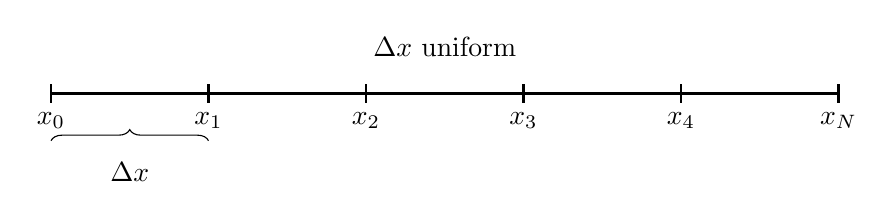
\begin{tikzpicture}[scale=1.0, >=Latex]
  \draw[thick] (0,0) -- (10,0);
  \foreach \i/\lab in {0/0,2/1,4/2,6/3,8/4,10/N}{
    \draw[thick] (\i,0.12) -- (\i,-0.12);
    \node[below] at (\i,-0.12) {$x_{\lab}$};
  }
  \node[above] at (5,0.35) {$\Delta x$ uniform};
  \draw[decorate, decoration={brace, amplitude=4pt}] (0,-0.6) -- (2,-0.6);
  \node[below] at (1,-0.75) {$\Delta x$};
\end{tikzpicture}
\end{center}
\end{frame}

% -------------------------
\begin{frame}{FTCS: Forward Time, Centered Space}
Approximate derivatives at $(x_i,t^n)$:
\[
\frac{\partial T}{\partial t}\Big|_{i,n} \approx \frac{T_i^{n+1}-T_i^{n}}{\Delta t},
\qquad
\frac{\partial^2 T}{\partial x^2}\Big|_{i,n} \approx \frac{T_{i+1}^{n}-2T_i^{n}+T_{i-1}^{n}}{(\Delta x)^2}.
\]

Insert into the 1D heat equation:
\[
\frac{T_i^{n+1}-T_i^{n}}{\Delta t}
=
\alpha\,\frac{T_{i+1}^{n}-2T_i^{n}+T_{i-1}^{n}}{(\Delta x)^2}
+\frac{S_i^n}{\rho c}.
\]

Define the diffusion number
\[
\lambda = \frac{\alpha\,\Delta t}{(\Delta x)^2}.
\]

\textbf{Explicit update (interior nodes):}
\[
T_i^{n+1} = T_i^{n} + \lambda\left(T_{i+1}^{n}-2T_i^{n}+T_{i-1}^{n}\right) + \Delta t\,\frac{S_i^n}{\rho c}.
\]
\end{frame}

% -------------------------
\begin{frame}{Interpretation: stencil = local energy balance}
Rewrite the update to highlight ``in minus out'':
\[
T_i^{n+1} = (1-2\lambda)T_i^n + \lambda T_{i-1}^n + \lambda T_{i+1}^n + \Delta t\,\frac{S_i^n}{\rho c}.
\]

\begin{itemize}
  \item $\lambda T_{i\pm 1}^n$ are contributions from neighbors (\emph{heat diffuses in}).
  \item $-2\lambda T_i^n$ is the net \emph{outflow} contribution.
  \item $\Delta t\,S/(\rho c)$ raises temperature when $S>0$.
\end{itemize}

If $S=0$, the update is a weighted average (plus the old value) \emph{only if} $\lambda$ is not too large.
\end{frame}

% -------------------------
\begin{frame}{Stability: why FTCS needs a time-step restriction}
For the 1D diffusion equation with $S=0$, von Neumann analysis gives
\[
0 \le \lambda \le \frac{1}{2}
\qquad \Longleftrightarrow \qquad
\Delta t \le \frac{(\Delta x)^2}{2\alpha}.
\]

\begin{itemize}
  \item Physically: you cannot let diffusion move information ``too far'' in one explicit step.
  \item Numerically: if $\lambda$ is too large, high-frequency modes grow $\Rightarrow$ oscillation/blow-up.
\end{itemize}

\vspace{0.5em}
Rule of thumb for class demos: pick $\lambda \approx 0.25$.
\end{frame}

% -------------------------
\begin{frame}{Algorithm slide (what students will code)}
Given $\alpha,\,\Delta x,\,\Delta t,\,N$ and initial data $T_i^0$:

\begin{enumerate}
  \item Compute $\lambda=\alpha\Delta t/(\Delta x)^2$ and ensure $\lambda\le 1/2$.
  \item For $n=0,1,2,\dots$:
  \begin{enumerate}
    \item Enforce boundary conditions to obtain $T_0^n$ and $T_N^n$.
    \item For $i=1,\dots,N-1$ update
    \[
    T_i^{n+1} = T_i^{n} + \lambda\left(T_{i+1}^{n}-2T_i^{n}+T_{i-1}^{n}\right) + \Delta t\,\frac{S_i^n}{\rho c}.
    \]
  \end{enumerate}
\end{enumerate}

\vspace{0.5em}
\textbf{Next lecture:} implicit methods $\Rightarrow$ linear systems (tridiagonal) and the Thomas algorithm.
\end{frame}

% -------------------------
\begin{frame}{One-slide recap}
\begin{align*}
\textbf{Balance law:}\quad
&\frac{\mathrm{d}}{\mathrm{d} t}\int_{\Omega}\rho cT \,\mathrm{d} V
= -\int_{\Gamma}\bq\cdot\bn \,\mathrm{d} S + \int_{\Omega} S \,\mathrm{d} V\\[0.25em]
\textbf{Divergence theorem:}\quad
&\int_{\Gamma}\bq\cdot\bn \,\mathrm{d} S=\int_{\Omega}\Div\bq\,\mathrm{d} V
\;\Rightarrow\;
\rho c\,T_{,t}+\Div\bq-S=0\\[0.25em]
\textbf{Fourier law:}\quad
&\bq=-k\Grad T
\;\Rightarrow\;
T_{,t}=\alpha\nabla^2T+\frac{S}{\rho c}\\[0.25em]
\textbf{FTCS (1D):}\quad
&T_i^{n+1} = T_i^{n} + \lambda\left(T_{i+1}^{n}-2T_i^{n}+T_{i-1}^{n}\right)+\Delta t\,\frac{S_i^n}{\rho c},
\quad
\lambda\le \tfrac12
\end{align*}
\end{frame}

\end{document}
